\documentclass[a4paper]{scrartcl}
\usepackage{fancyhdr}
\pagestyle{fancy}
\usepackage[english]{babel}
\usepackage[utf8]{inputenc}
\usepackage{graphicx}
\usepackage{url}
\usepackage{textcomp}
\usepackage{amsmath}
\usepackage{lastpage}
\usepackage{pgf}
\usepackage{wrapfig}
\usepackage{fancyvrb}

\usepackage{tikz}
\usetikzlibrary{arrows.meta, positioning}

% Listing header

\usepackage{listings}
\usepackage{xcolor}

\definecolor{lightgray}{gray}{0.95}

\lstdefinestyle{javastyle}{
    backgroundcolor=\color{lightgray},
    basicstyle=\ttfamily\small,
    numbers=left,
    numberstyle=\tiny,
    numbersep=8pt,
    frame=single,
    showstringspaces=false,
    breaklines=true,
    breakautoindent=true,
    breakindent=2em,
    keepspaces=true,
    columns=fullflexible,
    tabsize=4,
    language=Java,
    keywordstyle=\color{blue},
    commentstyle=\color{gray!70},
    stringstyle=\color{orange!90!black}
}

% Create header and footer
\headheight 27pt
\pagestyle{fancyplain}
\lhead{\footnotesize{Object-Oriented Design, IV1350}}
\chead{\footnotesize{Seminar 2 Solution}}
\rhead{}
\lfoot{}
\cfoot{\thepage\ (\pageref{LastPage})}
\rfoot{}

% Create title page
\title{Seminar 2}
\subtitle{Object-Oriented Design, IV1350}
\author{Mo Wang mowang@ug.kth.se}
%\date{\today} Prints today's date
\date{2026-03-30}

\begin{document}

\maketitle
\noindent\textbf{Project Members:} \\ \hfill
% \tableofcontents %Generates the TOC
[Mo Wang, mowang@ug.kth.se]

\section*{Declaration:}

By submitting this assignment, it is hereby declared that all group members listed above have contributed to the solution. It is also declared that all project members fully understand all parts of the final solution and can explain it upon request.

It is furthermore declared that no part of the solution has been copied from any other source (except for resources presented in the Canvas page for the course IV1350), and that no part of the solution has been provided by someone not listed as a project member above.

\section{Introduction}
\label{sec:intro}

% \textbf{This chapter tells \texttt{what} are you going to do.} Explain the task and the requirements on the solution. It's important to clearly state the requirements.

This report focuses on the \texttt{Design phase} of the \texttt{Repair Electric Bike} system and includes the design method, interaction diagrams, the resulting class diagram, and an evaluation of the design against the assessment criteria. The system design is based on the given requirements specification with both normal and alternative workflow scenarios, as well as following the \texttt{Domain Model} and \texttt{System Sequence Diagram} established earlier. The details of these diagrams can be found in Appendices~\ref{appendix:background}, \ref{appendix:domain-model} and \ref{appendix:system-sequence-diagram}.

\subsection{Requirements of Seminar 2}
The requirements of Seminar~2 are to design a complete, well-structured object-oriented architecture for the \texttt{Repair Electric Bike} system. The seminar focuses on applying established principles from the course literature, in particular Section~4.1 and Chapter~5 of \texttt{A First Course in Object-Oriented Development}.

The design must satisfy the following requirements:

\begin{itemize}
  \item \textbf{Layered architecture following the MVC and Layer patterns}.  
        The program must be organised into appropriate layers with correct 
        direction of dependencies and no mixing of responsibilities.

  \item \textbf{High cohesion, low coupling, and strong encapsulation}.  
        The design shall demonstrate a well-defined public interface, clear 
        responsibilities, and minimal dependencies between components.

  \item \textbf{Complete coverage of the entire Repair Electric Bike scenario}.  
        All basic and alternative flows must be designed, including the 
        startup sequence (the \texttt{main} method).

  \item \textbf{Interaction diagrams for all behaviour}.  
        The Result chapter must include sequence or communication diagrams 
        covering \emph{every} system operation, including alternative flows 
        and the startup sequence.

  \item \textbf{A class diagram consistent with the interaction diagrams}.  
        The diagram must include all classes used in the design, but may 
        omit excessive detail for clarity.
\end{itemize}

Implementation of the user interface and data persistence layer is out of scope. A simplified \texttt{View} class and a minimal integration layer are therefore used.

This report therefore describes the design method, the resulting class and interaction
diagrams, and a discussion evaluating the design according to the required principles.

\section{Method}
% \textbf{This chapter tells \texttt{how} you solved the task.} Explain how you worked and what tools you used when solving the tasks. \texttt{Do not explain your solution and do not present entire sub-results in detail. It's enough to explain which steps you performed and perhaps give a short example.} For example, some of the things to explain in the report for seminar one, is that you used a category list and noun identification to find class candidates for the domain model, and to tell which UML editor you used.

% Goal: Explain how you worked (not the solution itself)

Based on the domain model (DM) and system sequence diagram (SSD) from analysis, the system design can be carried out by first dividing the system into the layered architecture pattern based on MVC and therefore designing one system operation at a time while aiming high cohesion, low coupling and high degree of encapsulation. 

\subsection{Step 1. Use the patterns MVC and layer}

The first step involves usage of layered architectural MVC pattern, which includes several layers: view, controller, model, integration, data and startup, which can be visualized in Figure~\ref{fig:layered-architecture} showing a package diagram. It shows the different layers, where each of them has a clear responsibility and only interacts with the layer beneath it, following the direction of the dependencies illustrated in Layer pattern. 

View layer concerns interactions with user while core logic is handled in model layer. Controller layer acts as a bridge between the view and the model and carries the necessary system operations. By calling each system operation, the equivalent operations in the model and integration are handled. The integration layer acts as a middle ground between the core logic and data layer, which in turn is responsible for storing data. Finally, the startup layer handles program initialization of the rest five layers and serves as the main function.

% todo (Finished): please replace it using Astah package diagram. Do forget to add figure caption.

\begin{figure}[h!]
  \begin{center}
    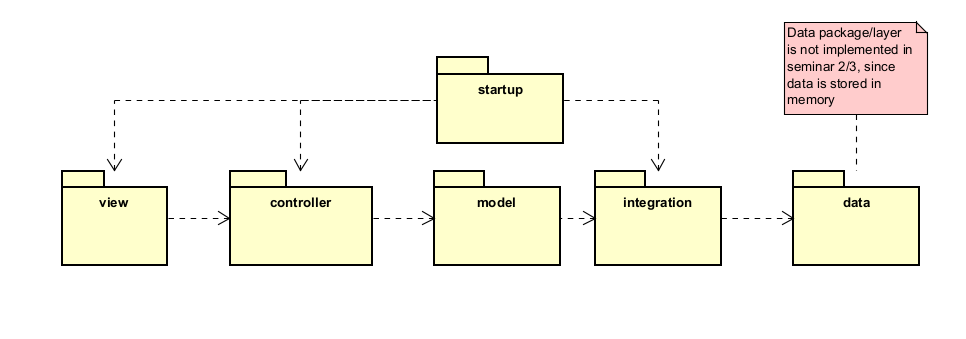
\includegraphics[width=\textwidth]{figures/package-diagram.png}
    \caption{The layered MVC architecture pattern is divided in layers with each package corresponding to each layer}
    \label{fig:layered-architecture}
  \end{center}
\end{figure}

The \texttt{bike repair system} implements the MVC pattern by dividing the entities in domain model as classes into different layers. Both View and Controller layer introduces its own classes, such as \texttt{ReceptionistController} and \texttt{TechnicianController} in Controller for different authorization roles, as well as \texttt{ControllerCreator} that centralizes controller class constructions.

% todo (Finished): controller, only provides findRepairOrder which would be used by R and T.
% todo (Finished): ControllerCreate
% todo: update Astah class diagram to add ControllerCreater, RegistryCreator.

\subsection{Step 2. Design one system operation at a time}
During the design process of the system, each system operation is analyzed into its corresponding interaction diagram. These diagrams illustrates the flow of execution and the order of execution in an enumerated sequence and provides visualization on how messages are passed between objects, unlike class diagrams which primarily visualizes static system relationships.

In this case, communication diagrams are used since they offer more compact view, instead of sequence diagrams because sequence diagrams occupy large amount of space and become complex when tracing the flow of messages across different class instances. On the other hand, communication diagrams ephasizes the relationships between objects and exchanged messages. 

Designing each sequence diagram for each system operation begins by creating the necessary class instances as well as the main instance from View class to a Controller class. etc.

A typical system operation begins with a call from the View to the Controller, which then delegates work to Model and Integration objects following the message flow in the SSD. For instance, the \texttt{searchCustomer} operation can be visualized as a sequence diagram by tracing the method calls across layers: starting from the \texttt{View} class calling \texttt{searchCustomer} on the \texttt{ReceptionistController}, which in turn interacts with the relevant classes in the Model and Integration layers to look up the customer data.

% todo (Finished): add last paragraph with one sentece, use Astah as tool to ...

The communication diagrams for each system operation are drawn and visualized using Astah tool, which is specialized for UML diagram design. The tool helps to design a structured and standardized UML representation of interactions as well as easier modification of diagrams and improved consistency across the system design process.

\subsection{Step 3. High cohesion, low coupling, and a high degree of encapsulation with a small, well-defined public interface }
High cohesion, low coupling, and a high degree of encapsulation with a small, well-defined public interface are several important OOD guidelines.

When a new functionality is added, method should only be created that these principles are satisfied as fully as possible. For instance, a class or a method should be responsible for its dedicated and solemn functionality with as few connections to its neighbour classes as possible.

For achieving high degree of encapsulation, some internal helper functions that works inside a class should be hidden if it doesn't contribute to connection with other classes. As an example, helper methods such as the phone-format conversion inside \texttt{TelephoneNumber} are kept private, because no class outside that type needs access.

Additionally, each operation is placed in the class that represents its abstraction with the necessary data for the operation. The domain model can be used to identify potential new classes that may need to be introduced.

Objects are favoured over primitive data types as well as avoiding static members, since primitive data and static members are not object oriented which causes harder to achieve these three guidelines. For instance, \texttt{Cost} is modeled as its own class instead of using primitive numbers, since cost include amount, currency and probably future metadata.

% todo (Finished): only one sentence for example.

\subsection{Step 4. Class diagram for relationship between classes}
After designing system operation sequence diagrams and considering the three OOD guidelines, class diagram for relationship can be drawn by adding all classes that has been used in sequence diagrams and add them into the class diagram. Each class is placed into its corresponding package, where each package maps into a layer, with lines connecting the class relationships.

The class diagram is also drawn using Astah tool, since it provides efficient support for organizing classes into packages, visualizing relationships clearly, and maintaining a consistent UML design.

% todo (Finished): add last paragraph with one sentece, use Astah as tool to ...

\subsection{Step 5. Implement the new design in code}
In the last step, the new design in code is implemented, with the help from class diagram and sequence diagrams for each operation. The class diagram helps to create the skeleton code with each class name, whereas the system operation helps to write the implementation of each system operation. The design is implemented in code to verify that the interactions and dependencies defined in the diagrams were feasible.

By implementing the design in code, the code editor VSCode is used since it offers syntax highlightening and autocompletion. For compiling and testing the code, Maven is used for full codebase compilation, handle project dependencies and automate build tasks as well as integrating testing using JUnit test cases.

% todo (Finished): add last paragraph with one sentece, use vscode to edit coding, use mvn to compile and test coding.

\section{Result}
\label{sec:result}

% \textbf{This chapter explains \texttt{the result} of what you did.} \textbf{The report must show that you have done the work yourself and that you have understood what you have done}, both of these goals are met by explaining your solution here in the result chapter. All figures must be referenced in the text. Ask yourself if the solution is clearly explained, and if the reader will understand the application. What would you yourself want to know if you read about the application, is that included in the report? More specific instructions for the content can be found in each assignment.

Following the method's steps, sequence diagrams for each system operation and class diagrams are created. These diagrams serve as blueprints for the subsequent implementation.

The system adopts a layered architecture based on the MVC pattern, where each layer is mapped to a corresponding package. Since the project includes internal computational logic, database or file operations, and an interactive user interface, the program is divided into layers that each handle a specific concern. This separation allows responsibilities to be clearly partitioned—for example, the data layer manages file operations, while the model layer handles internal computation.

Every system operation defined in the SSD is converted into a communication diagram, presented in the same order as in the SSD. The first operation, searchCustomer, retrieves a customer using a telephone number as input. It should also be noted that the view package is not fully designed at this stage. Instead, it contains only a placeholder class, View, representing a future user interface.

\subsection{The \texttt{searchCustomer} system operation}

In the searchCustomer case, the \texttt{View} class calling the method \texttt{searchCustomer} with a phone number in free format on \texttt{ReceptionistController} can be first written. Since a customer object needs to be returned, the receptionist controller class should find the corresponding customer. This can be done by calling \texttt{CustomerRegistry} that stores and handles customer informations, the function \texttt{find} is called by passing a phone number in canonical E164 format. In this case, the given phone must be converted from any format into canonical E164 format through \texttt{TelephoneNumber} class, before handing it into CustomerRegistry. The full process of is visualized in Figure~\ref{fig:search-customer}.

\begin{figure}[h!]
  \begin{center}
    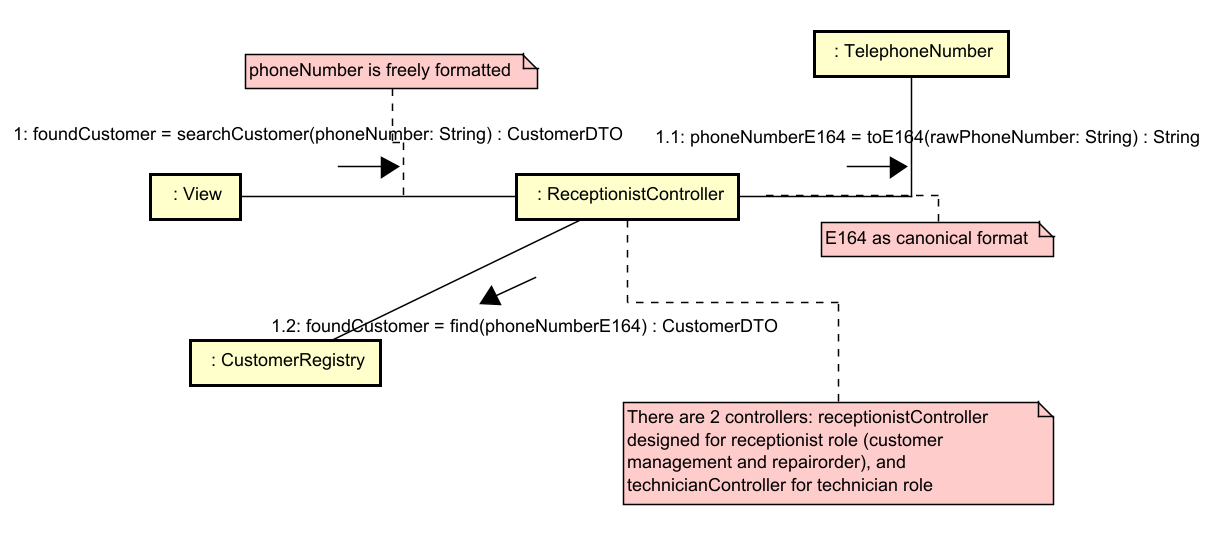
\includegraphics[width=\textwidth]{figures/sequence-diagram-1.png}
    \caption{A communication diagram for \texttt{searchCustomer} system operation}
    \label{fig:search-customer}
  \end{center}
\end{figure}

% todo (Finished): The start sequence in the main method, the figure should be added.

Additionally, in order for the program to produce results, the start sequence must also be implemented. During initialization, all relevant classes in each layer should be initialized during startup. This includes initializing \texttt{RegistryCreator}, \texttt{Printer}, \texttt{ControllerCreator} and \texttt{View} class which represents the fundamental classes of each layer. In integration layer, \texttt{RegistryCreator} starts up \texttt{CustomerRegistry} and \texttt{RepairOrderRegistry}, as well as \texttt{ControllerCreator} starting up \texttt{TechnicianController} and \texttt{ReceptionistController}.

\begin{figure}[h!]
  \begin{center}
    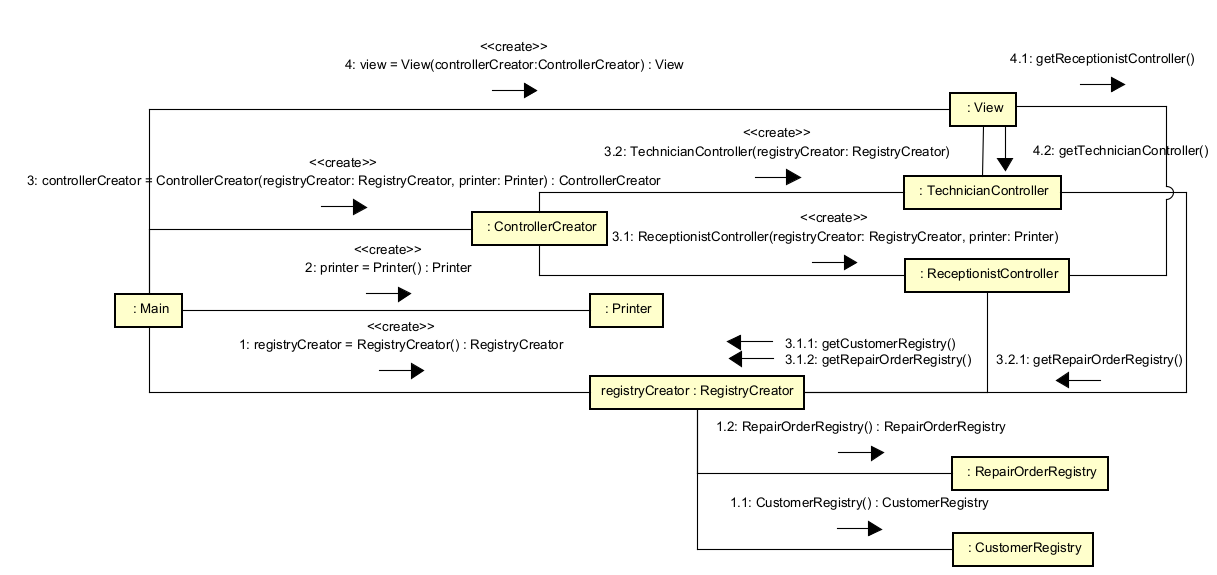
\includegraphics[width=\textwidth]{figures/startup.png}
    \caption{A simplified and tailored diagram for program startup after implementing \texttt{searchCustomer} system operation. this diagram only illustrates the subset of classes used in this operation of startup, but only shows the relevant classes for the current system operation.}
    \label{fig:startup}
  \end{center}
\end{figure}

% Old words are commented out. May recover if necessary
% During developing the system, there are problems in terms of guidelines, and how these are resolved:
% Some class can both be designed as a DTO or as an entity, which raises ambigouisty. To address this problem, classes that has fields that does not update during program execution are assigned as DTO, such as customer and bike. On the other hand, classes that updates during execution are kept as entities, but converts into DTO when the Controller layer handing over the class to View layer.

% Additionally, some fields are assigned with an object type instead of primitive value, for example \texttt{Cost} class. The reason is that \texttt{Cost} class both contains an amount and a currency, which cannot be stored together as one variable as primitive values. This lowers coercion and causes unnecessary coupling, since classes with costs needs extra logic to handle both variables, as well as difficulties in extending cost attributes. 
% However, in some cases, a primitive value is preferred such as telephone number and email adress. The reason is that telephone numbers has a fixed format which fits perfectly into a primitive type. Since telephone numbers rarely experience format changes, a separate class would involve redundant complexity.


In the \texttt{searchCustomer} operation several important design principles are applied, including encapsulation with a small, well-defined public interface, high cohesion and low coupling. First, the telephone number provided by the view is accepted in any arbitrary format, but must be normalized by converting into canonical E164 form in the method \texttt{toE164} in \texttt{TelephoneNumber} class. This ensures that data does not "appear out of nothing" and that both original and transformed values are explicit written.

Both \texttt{CustomerDTO} and \texttt{BikeDTO} are immutable DTO classes located in the integration layer. This prevents the view from receiving references to mutable class objects and ensures strong encapsulation. Using the same object name throughout the interaction diagram makes it clear that the same instance is passed across layers, which simplifies understanding of the data flow.

Cohesion is increased since each class performs only the task it is intended for: \texttt{TelephoneNumber} formats numbers, \texttt{CustomerRegistry} retrieves customer information, and the controller coordinates flow without performing logic. Coupling is minimized by ensuring that the controller does not take responsibility in customer storage, nor how telephone numbers are validated.

The class diagram is maintained that includes all relevant classes. Classes and their relationships are added progressively as sequence diagrams for each system operation are developed. However, certain classes, such as data transfer objects (DTOs), may be omitted, along with attributes that are not relevant or contribute little to the understanding of the design.

For instance, in Figure~\ref{fig:class-diagram-search-customer}, the class diagram includes the relevant classes involved in the searchCustomer system operation illustrated in Figure~\ref{fig:search-customer}.

\begin{figure}[h!]
  \begin{center}
    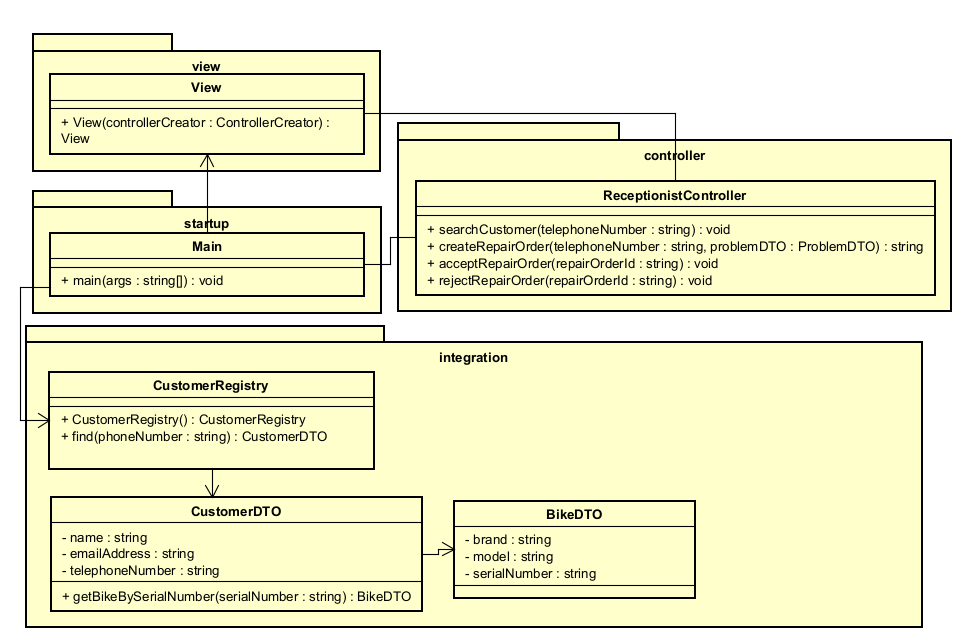
\includegraphics[width=\textwidth]{figures/class-diagram1.png}
    \caption{A class diagram with relevant classes that is involved in \texttt{searchCustomer} system operation. The diagram does not show the layout of final class diagram.}
    \label{fig:class-diagram-search-customer}
  \end{center}
\end{figure}


\subsection{The \texttt{createRepairOrder} system operation}

The \texttt{createRepairOrder} system operation can be translated by identifying the operation steps. The operation starts with searching the broken bike from bike serial number and creating a \texttt{ProblemDTO} with description and the found broken bike. Afterwards, the \texttt{ProblemDTO} is passed to \texttt{ReceptionistController} which first fetch its corresponding customer and therefore creates a \texttt{RepairOrder} which is saved later in \texttt{RepairOrderRegistry}. These steps are visualized in Figure~\ref{fig:create-repair-order}.

The \texttt{createRepairOrder} operation builds on the DTO-policy established in the design. \texttt{ProblemDTO} is used as input because it represents a snapshot of customer problem data that may expand in future (e.g.\ urgency or additional flags). Using a DTO instead of several primitive parameters avoids long parameter lists and preserves low coupling and a stable public interface.

\texttt{RepairOrder} is a mutable entity in the model layer. Its state evolves as diagnostics and tasks are added later in the workflow. Meanwhile, \texttt{CustomerDTO} and \texttt{BikeDTO} are immutable because customer and bike data do not change during program execution. This clear separation between entity and DTO avoids ambiguity and prevents leaking modifiable internal state to external layers.

Encapsulation is maintained by ensuring that the controller does not directly modify the internals of a \texttt{RepairOrder}. Instead, it delegates to the model, which contains the logic for constructing and validating a new repair order. Coupling is reduced because only \texttt{RepairOrderRegistry} handles data persistence, while \texttt{ReceptionistController} only forwards the ProblemDTO and orchestrates the operation.

\begin{figure}[h!]
  \begin{center}
    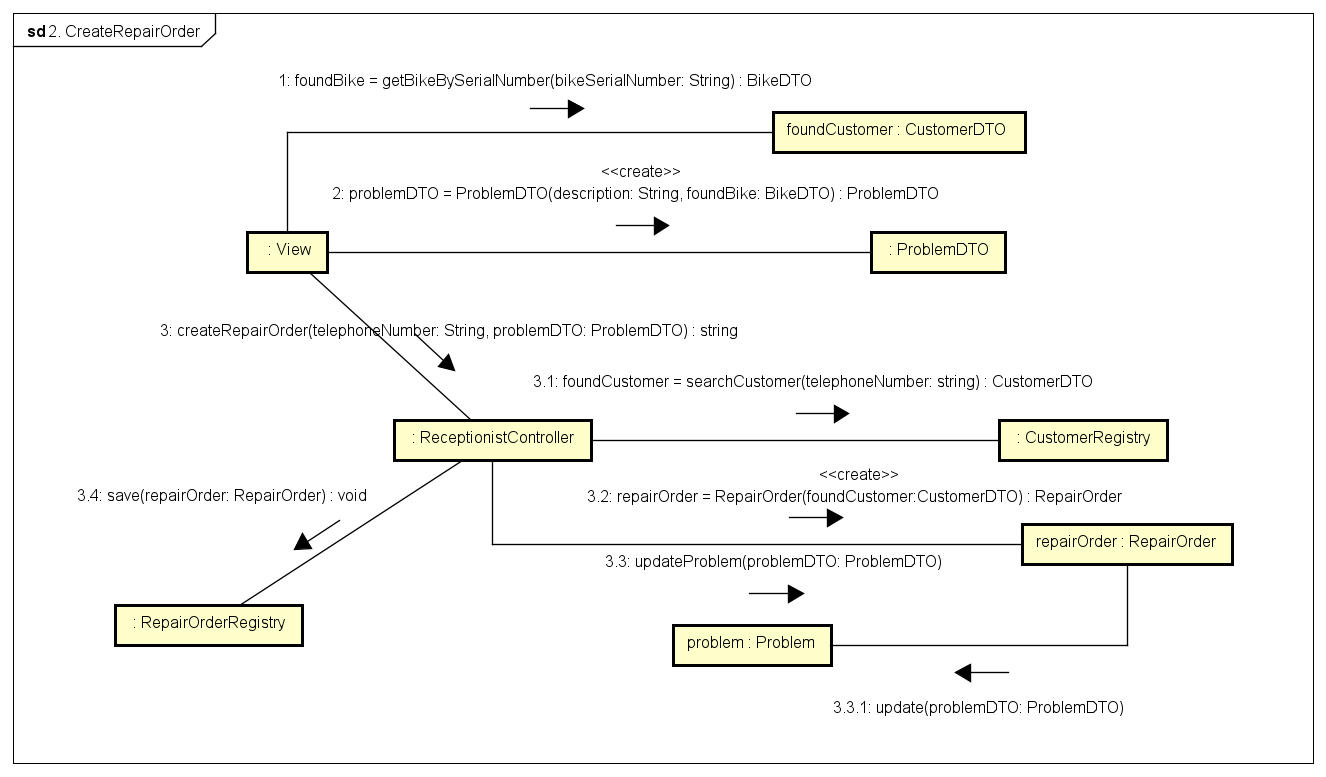
\includegraphics[width=\textwidth]{figures/sequence-diagram-2.png}
    \caption{A communication diagram for \texttt{createRepairOrder} system operation}
    \label{fig:create-repair-order}
  \end{center}
\end{figure}


\subsection{The \texttt{findRepairOrder} system operation}
The \texttt{findRepairOrder} system operation finds the most recent created repair order of a customer. This is done by first fetching all the repair orders filtered by a given telephone number, and the most recent added repair order is selected. The telephone number used to retrieve the repair order comes directly from user input or a previous interaction. The system operation is visualized in Figure~\ref{fig:find-repair-order}.

To prevent exposing model internals, \texttt{RepairOrderRegistry} returns a \texttt{RepairOrderDTO} instead of the repair-order entity itself. The view is never allowed to receive a reference to a mutable \texttt{RepairOrder} object, in order to ensure strict encapsulation and protecting the consistency of the model state.

Cohesion is maintained because each class serves one purpose: the registry looks up stored orders, the entity encapsulates business logic, and the controller only coordinates the sequence of calls. Coupling is kept low because the controller does not know how orders are stored internally.

\begin{figure}[h!]
  \begin{center}
    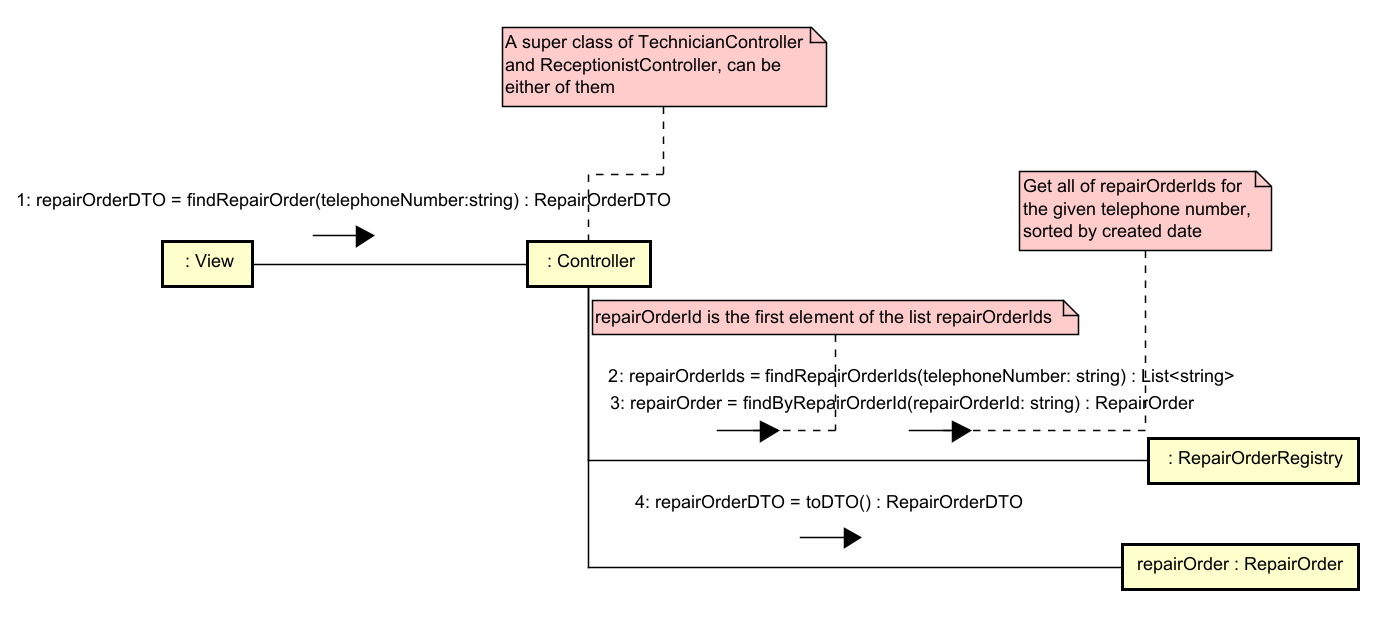
\includegraphics[width=\textwidth]{figures/sequence-diagram-3.png}
    \caption{A communication diagram for \texttt{findRepairOrder} system operation}
    \label{fig:find-repair-order}
  \end{center}
\end{figure}

\subsection{The \texttt{addDiagnosticResult} system operation}
The \texttt{addDiagnosticResult} system operation attaches a diagnostic result onto a repair order. The operation starts by creating a \texttt{ResultDTO} object that contains the description as well as \texttt{checked} flag for having the diagnostic task checked and \texttt{toBeRepaired} flag. Afterwards, the repair order and the diagnostic task are first fetched before updating the diagnostic result of the diagnostic task of the repair order as well as calculating the total cost of repair order and saving it back into its registry. The operation can be visualized in Figure~\ref{fig:add-diagnostic-result}.

Diagnostic results are added using a \texttt{DiagnosticReportDTO}, which is an immutable data carrier. The actual logic for incorporating the diagnostic report belongs to the \texttt{RepairOrder} entity, which updates its internal state through a dedicated method. This ensures that behavior, not the controller, performs the state change, preserving cohesion and encapsulation.

The DTO is never modified. Instead, all updates occur in the model, preventing attribute leakage. Coupling remains low because the controller does not need to know how diagnostic results are stored or validated. All validation and state management sits inside the model layer.

\begin{figure}[h!]
  \begin{center}
    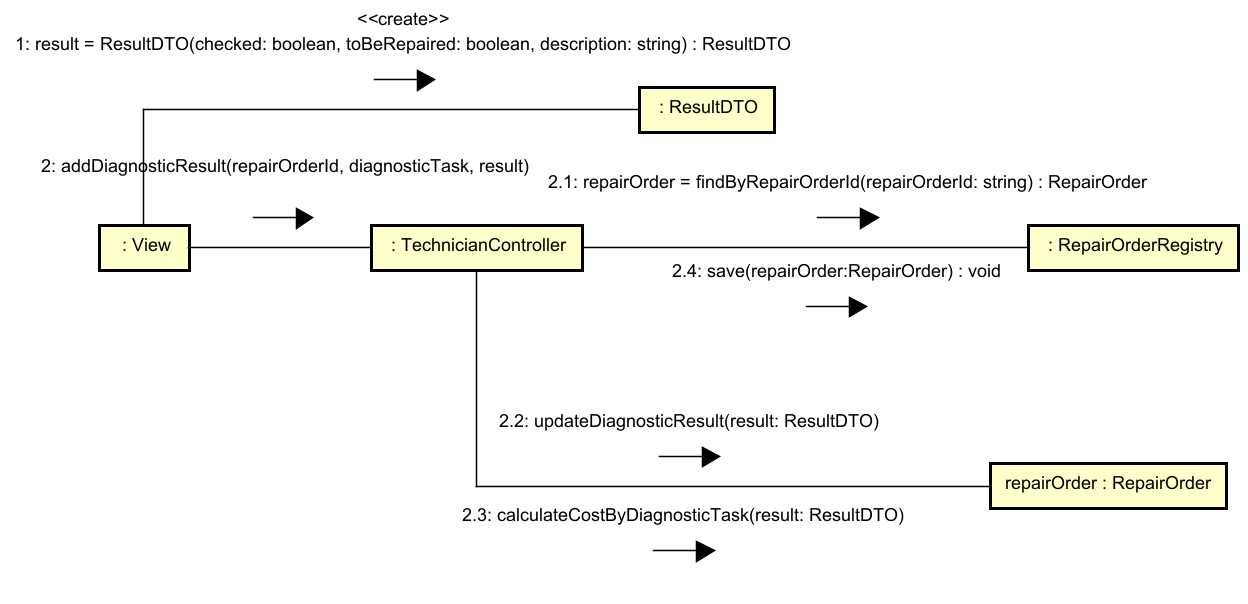
\includegraphics[width=\textwidth]{figures/sequence-diagram-4.png}
    \caption{A communication diagram for \texttt{addDiagnosticResult} system operation}
    \label{fig:add-diagnostic-result}
  \end{center}
\end{figure}

\subsection{The \texttt{createProposedRepairTask} system operation}
In Figure~\ref{fig:create-proposed-repair-task}, the \texttt{createProposedRepairTask} system operation creates a new proposed repair task for a repair order. First, a \texttt{ProposedRepairTaskDTO} is created containing name, description, cost and estimated finish time in days. The DTO object is then attached to a repair order by first fetching the given repair order using a \texttt{repairOrderId}, as well as updating the total cost of the repair order. Finally, the operation ends with saving the repair order in its registry.

Each proposed task is encapsulated inside a \texttt{ProposedRepairTaskDTO}, which contains immutable data. The task is added to the repair order through a method belonging to the \texttt{RepairOrder} entity. This keeps all business behavior inside the model layer and prevents the controller from internal logic responsibilities.

A dedicated \texttt{Cost} class is used instead of primitive values. This avoids overuse of primitive values which can increases cohesion by grouping related values and reduces coupling by centralizing cost-related logic in a relevant class. Since the DTO is immutable, objects are kept intact and never hand out modifiable references.

\begin{figure}[h!]
  \begin{center}
    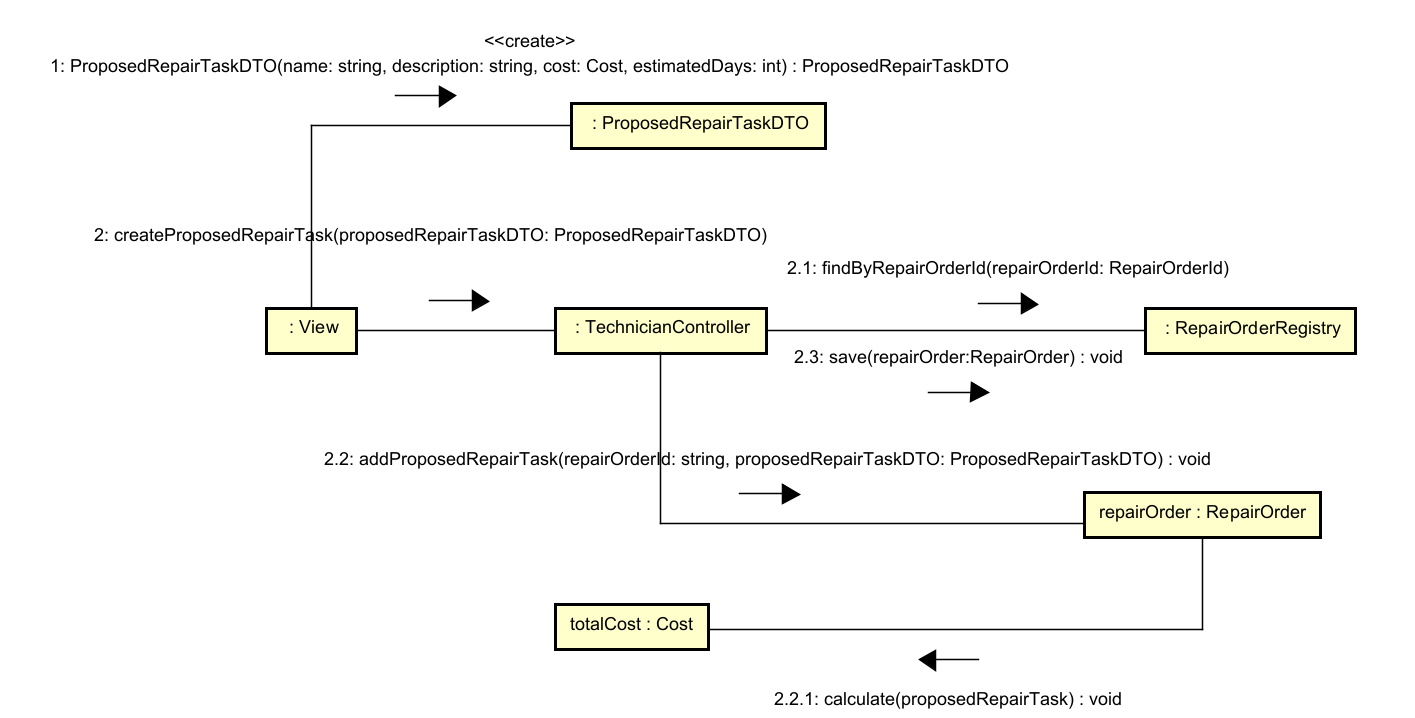
\includegraphics[width=\textwidth]{figures/sequence-diagram-5.png}
    \caption{A communication diagram for \texttt{createProposedRepairTask} system operation}
    \label{fig:create-proposed-repair-task}
  \end{center}
\end{figure}

\subsection{The \texttt{acceptRepairOrder} system operation}
The \texttt{acceptRepairOrder} system operation accepts a repair order by a repairOrderId, as shown in Figure~\ref{fig:accept-repair-order}. The \texttt{RepairOrder} is first found from a \texttt{repairOrderId}, which an \texttt{accept} method is called for updating the repair order state to \texttt{Accepted}. The repair order is saved back to its registry, as well as printing out the repair order.

Accepting or rejecting a repair order is a state transition and therefore belongs to the \texttt{RepairOrder} entity. The controller only calls the corresponding method and does not implement any business logic itself.

Encapsulation is achieved by keeping the internal status field of repair order as private. Only well-defined public methods such as \texttt{accept()} and \texttt{reject()} can modify the state. The object is later returned to view as DTO ensuring that mutable entities are not passed to view. Coupling remains low since no external class needs to know how the state is represented internally.

\begin{figure}[h!]
  \begin{center}
    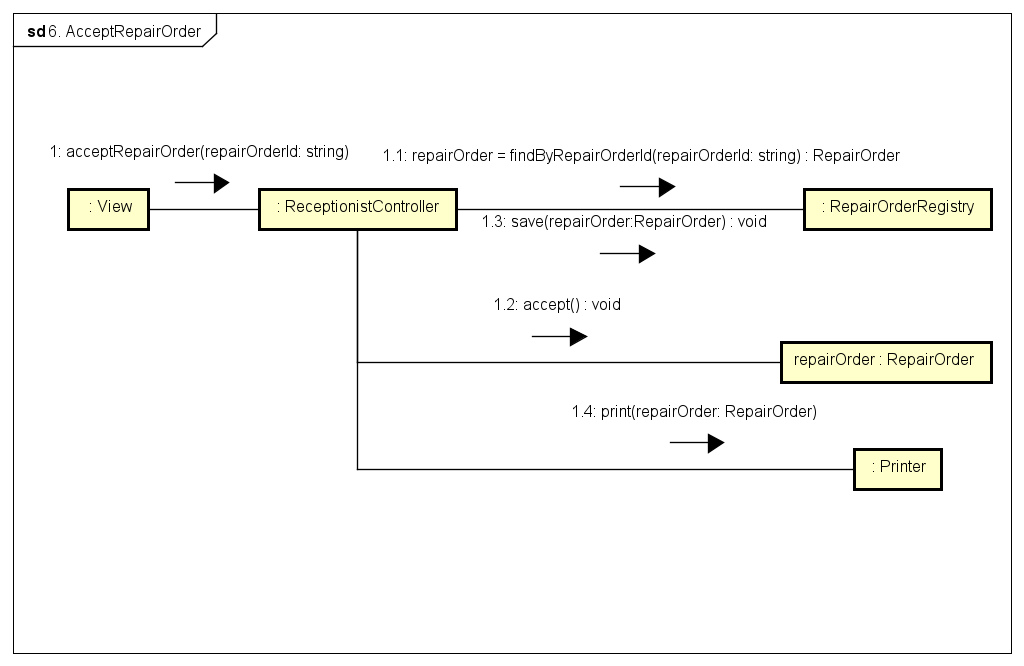
\includegraphics[width=\textwidth]{figures/sequence-diagram-6.png}
    \caption{A communication diagram for \texttt{acceptRepairOrder} system operation}
    \label{fig:accept-repair-order}
  \end{center}
\end{figure}

\subsection{The \texttt{rejectRepairOrder} system operation}
The \texttt{rejectRepairOrder} follows the same pattern as \texttt{acceptRepairOrder} system operation, but the receipt and reports are not printed out. The action steps for rejecting a repair order is visualized in Figure~\ref{fig:reject-repair-order}

\begin{figure}[h!]
  \begin{center}
    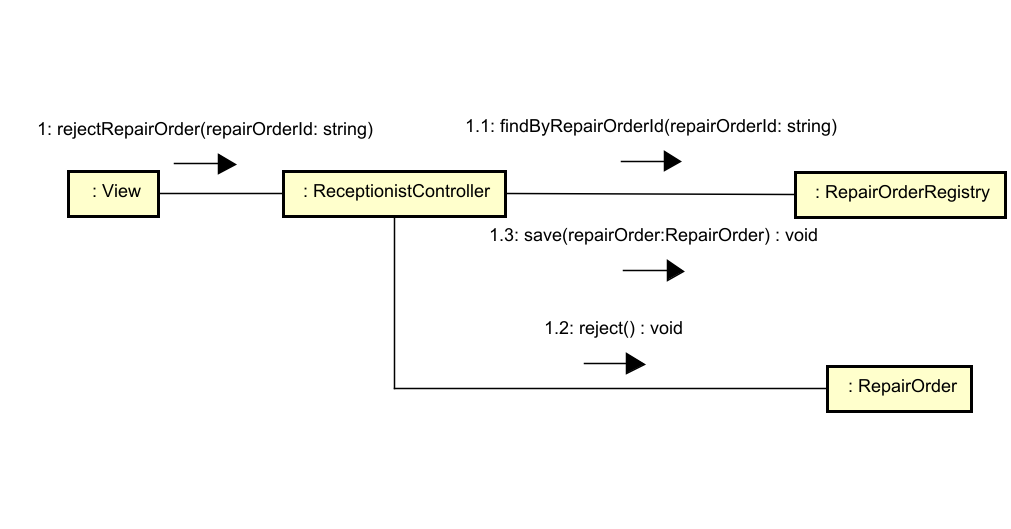
\includegraphics[width=\textwidth]{figures/sequence-diagram-7.png}
    \caption{A communication diagram for \texttt{rejectRepairOrder} system operation}
    \label{fig:reject-repair-order}
  \end{center}
\end{figure}

\subsection{Full communication diagram of \texttt{Startup}}

In startup procedure, given in Figure~\ref{fig:startup}, all entry classes in each layer should be initialized, in order for the program to be initialized. The classes includes creator classes such as \texttt{RegistryCreator} for integration layer and \texttt{ControllerCreator} for controller layer, as well as \texttt{View} which acts as an interactive interface to user. Additionally, \texttt{Printer} class which is located in integration layer is also be initialized.

Furthermore, in integration layer, \texttt{RegistryCreator} starts up \texttt{CustomerRegistry} and \texttt{RepairOrderRegistry}, as well as \texttt{ControllerCreator} initializes \texttt{ReceptionistController} and \texttt{TechnicianController}.


\begin{figure}[h!]
  \begin{center}
    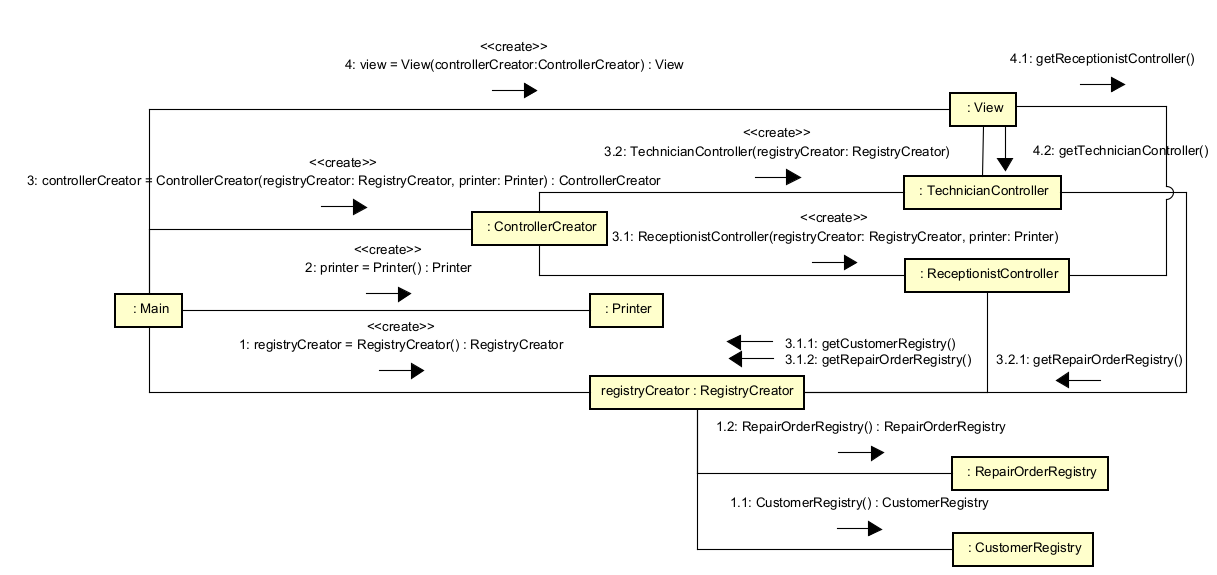
\includegraphics[width=\textwidth]{figures/startup.png}
    \caption{A full communication diagram for startup operation during program initialization. All entry classes of each layer are initialized.}
    \label{fig:startup}
  \end{center}
\end{figure}

\subsection{Full class diagram}

The full class diagram can be visualized in Figure~\ref{fig:class-diagram}, which represents a layered system architecture with five main packages: startup, view, controller, model, and integration. The data package is omitted since the program currently does not store any data into secondary storage, such as disk and database. Each package takes a specific and unambiguous responsibility inside the system, which ensures separation of concerns and maintainability.

\begin{figure}[h!]
  \begin{center}
    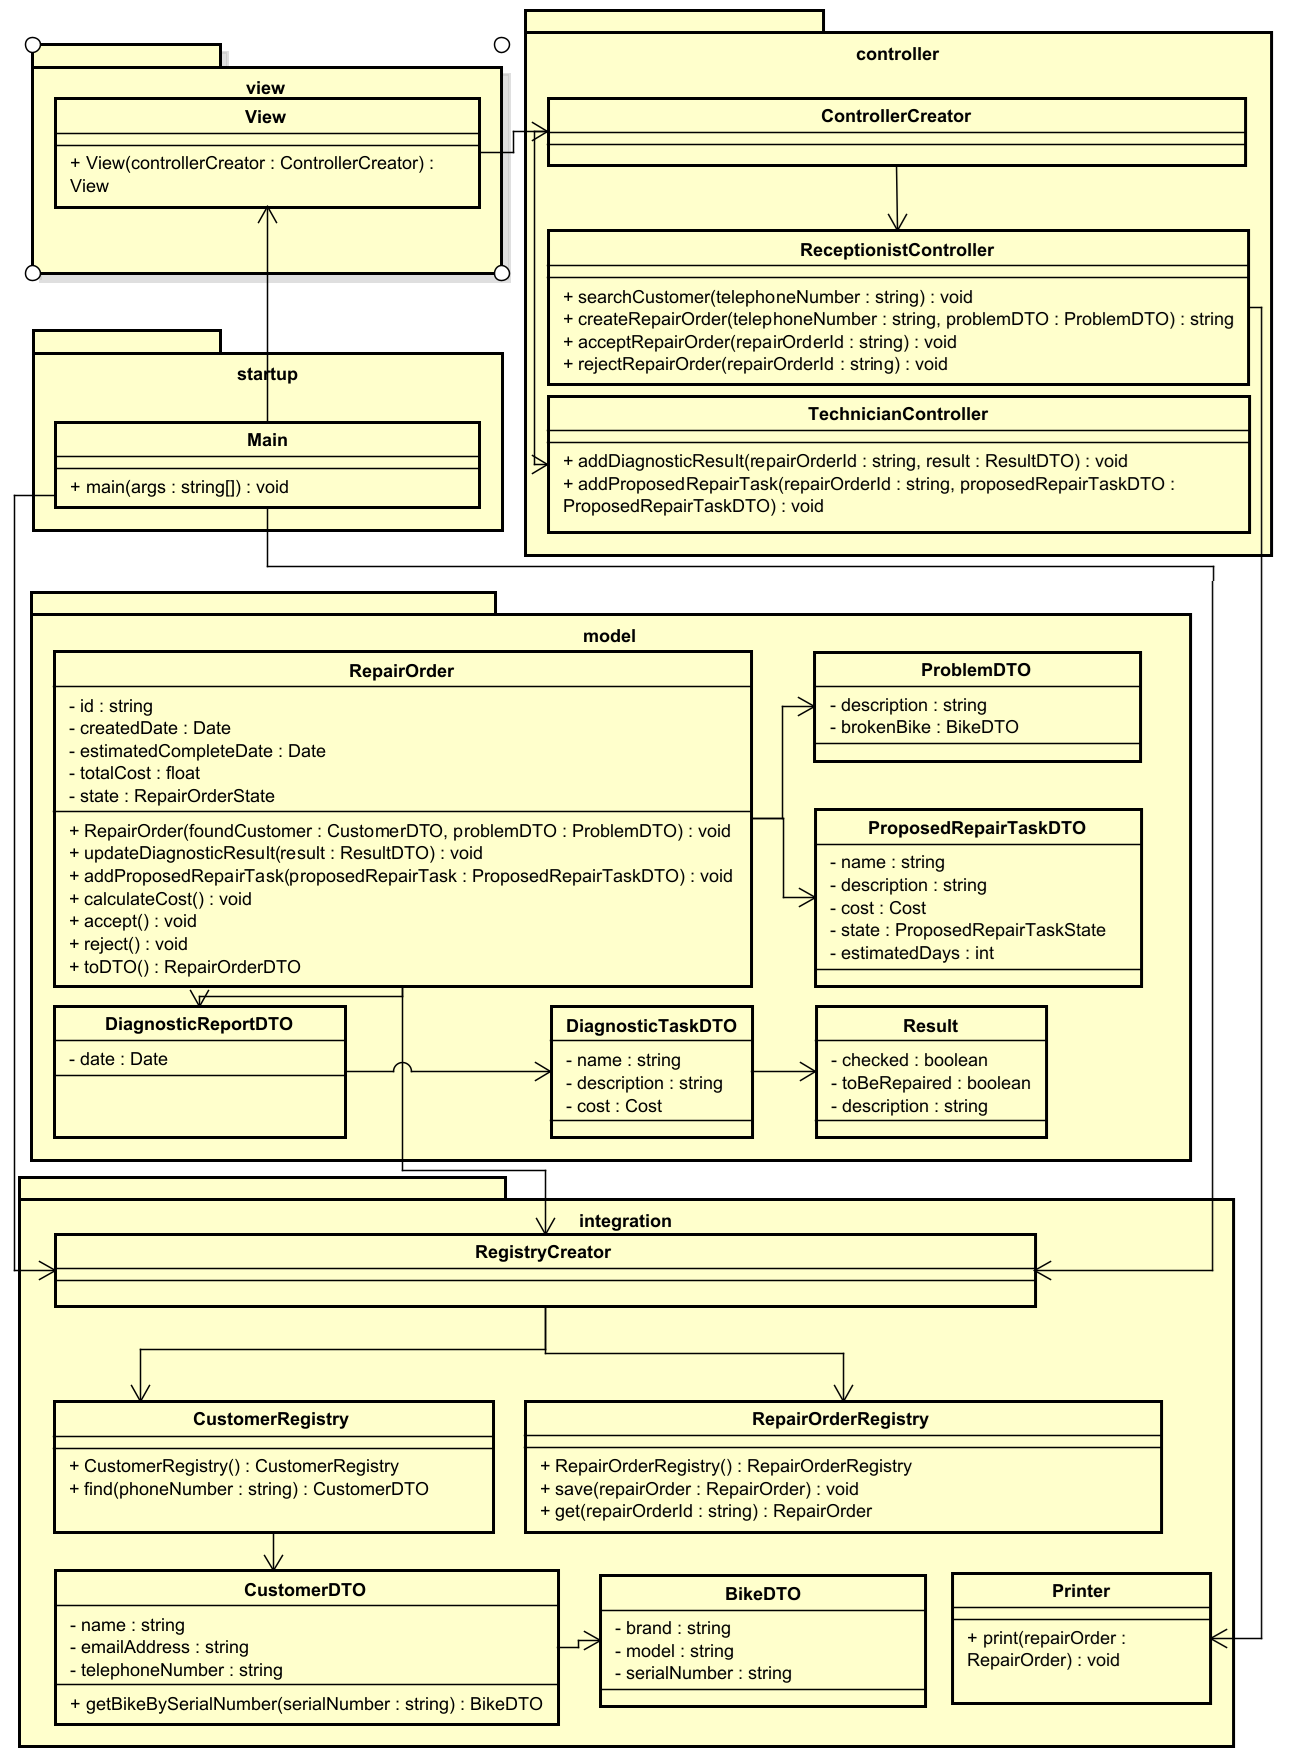
\includegraphics[width=\textwidth]{figures/class-diagram-i1.png}
    \caption{A sample diagram to illustrate caption (this text), numbering and reference in text.}
    \label{fig:class-diagram}
  \end{center}
\end{figure}

The startup package contains the \texttt{Main} class, which serves as the entry point of the application, initializing the necessary class instances.

The view package contains the \texttt{View} class, which acts as the user interface layer. Currently, the view class is hardcoded and communicates directly with the control layer by calling system operations as methods in classes of control layer.

The controller package acts as an intermediary control flow layer between the view and model layers. The abstract \texttt{Controller} class provides a shared \texttt{findRepairOrder}. Two subclasses are created for both \texttt{Receptionist} and \texttt{Technician}: \texttt{ReceptionistController} and \texttt{TechnicianController}. The \texttt{ReceptionistController} handles operations related to customer interaction, such as searching for customers, creating repair orders, and accepting or rejecting them. The \texttt{TechnicianController} manages diagnostic results and proposed repair tasks. Implementing each controller class for each role provides clear separation, while the base class for common logic.

The model package encapsulates the core computational logic. The central class is \texttt{RepairOrder}, which maintains repair order informations such as ID, date, cost, and state. It provides methods for updating diagnostic results, adding repair tasks, calculating cost, and changing the order state. Several supporting DTO classes are included, such as \texttt{ProblemDTO}, \texttt{ProposedRepairTaskDTO}, \texttt{DiagnosticReportDTO}, and \texttt{DiagnosticTaskDTO}, which serves as data encapsulations. The \texttt{Result} class represents the result of each diagnostic task.

The integration package acts as a middle-ground between model and data layer, which caches data from disk and database storage. The classes act as a middle ground, such as \texttt{CustomerRegistry} class that stores \texttt{CustomerDTO} instances provided with customer data, allowing lookup by phone number as well as \texttt{BikeDTO}. The \texttt{RepairOrderRegistry} manages storage and retrieval of \texttt{RepairOrder} objects. Additionally, \texttt{Printer} class is responsible for outputting repair order information.

\section{Discussion}

% \textbf{This chapter evaluates your solution} according to the assessment criteria found in the assessment-criteria documents, which are available under each seminar (sections 4.1-4.4) on the \texttt{Seminar Tasks} page of the course web. To get 2p, it's important that the evaluation is extensive, and \textbf{motivated with concrete examples from your solution}. General statements, that could be applied to any solution, will not contribute to a higher score.

\subsection{Evaluation of MVC Architecture, Layering, and Object-Oriented Design Quality}

% Are the MVC and Layer patterns used correctly? Are there enough layers? Enough packages? Enough classes? Does the controller handle any logic (it should not)?
% - Is there view-related code in the model (there should not be any)?
% - Is there low coupling, high cohesion and good encapsulation?
% - Is the use of low coupling, high cohesion and encapsulation explained in the report?

The design follows the MVC and Layer patterns, by separation into View, Controller, and Model. The View contains only user-interaction logic, which are currently hard-coded, while all system-operation logic is placed in the controllers, and business logic remains in the Model. Additionally, view-related code does not appear in other layer, which confirms that all the concerns are separated into layers that focus on one single, unambiguous responsibility.

Furthermore, the design contains all necessary layers: View, Controller, Model, Integration, and Startup. Multiple controller classes (\texttt{ReceptionistController} and \texttt{TechnicianController}) shows that there are enough classes to separate responsibilities, and none of the controllers contain core business logic, which stays consistent with the guideline that the controller does not take responsibility in granular and detailed core logic.
The Integration layer holds the DTOs and registry classes, ensuring that data access is completely separated from the model logic. This matches the Layer pattern expectations and maintains correct dependency flow.

The design produces high cohesion, low coupling, and good encapsulation. Cohesion is ensured since each class takes only one responsibility. For instance, \texttt{ProposedRepairTask} encapsulates only task description and cost while \texttt{RepairOrder} manages only repair-order state, diagnostic results, and repair tasks. Low coupling is achieved by ensuring that controllers depend only on registry interfaces and control flows, rather than internal implementation of model entities. As a result, model entities can evolve without affecting other layers. Encapsulation is strengthened through the consistent use of immutable DTOs, which prevent View from mutating internal states, as well as model objects never leak internal references, and all state transitions occur through dedicated domain methods rather than updating them externally.



The design produces high cohesion, low coupling, and good encapsulation.

Cohesion is ensured since each class takes only one single responsibility. For exqmple, \texttt{TelephoneNumber} is dedicated solely to validating and normalizing phone numbers, while \texttt{Cost} encapsulates amount and currency without mixing in additional behavior. Even supporting classes such as \texttt{Printer} focus strictly on formatting and printing repair-order summaries,
rather than performing any model or controller logic.

% todo: talk more about high cohesion (split up the model RepairOrder class -> ).
% For instance, \texttt{ProposedRepairTask} encapsulates only task description, cost, and estimated duration, while \texttt{RepairOrder} manages only repair-order state, diagnostic results, and attached repair tasks.

% todo: DO NOT COPY: Low coupling means there are as **few dependencies** as possible in the program

Low coupling is achieved by ensuring that controllers depend only on registry interfaces and high-level operations, rather than the internal implementation of model entities. For example, the \texttt{ReceptionistController} never inspects the internal fields of \texttt{RepairOrder}; instead, it calls well-defined model methods such as \texttt{accept()} or \texttt{addDiagnosticResult()}. Likewise, the \texttt{TechnicianController} does not need to know how proposed tasks are stored internally; it simply invokes \texttt{addProposedTask()} on \texttt{RepairOrder}. Because of this, model entities can evolve—such as replacing a list with a more advanced collection structure—without requiring any changes in controllers or the View.


% todo: Encapsulation means hiding a class’s internal details by exposing only its public interface while keeping private implementation code inaccessible to the rest of the program.
% your examples of public vs private.
Encapsulation is strengthened through the consistent use of immutable DTOs, which prevent the View from mutating internal system state. For instance, \texttt{CustomerDTO}, \texttt{BikeDTO}, and \texttt{RepairOrderDTO} expose only accessors, never mutators, ensuring that external layers cannot corrupt the model. Model objects also never leak internal references; for example, \texttt{RepairOrder} never exposes its internal task list directly. Instead, all state transitions occur through dedicated domain methods such as \texttt{addTask()}, \texttt{setDiagnosticReport()}, or \texttt{reject()}. This prevents accidental modification from outside the class and ensures that all invariants are checked within the model layer. Together, these choices result in a design where responsibilities are clear, coupling remains minimal, and the system maintains a strong and robust encapsulation boundary.

\subsection{Evaluation of Type Correctness, Object Usage, and Data Encapsulation}
% 4.2 Evaluation of Type Correctness, Object Usage, and Data Encapsulation
% - Are parameters, return values and types correctly specified? Is it clear from where values come?
% - Are objects used instead of primitive data as much as possible?
% - Are there static methods or attributes? If so, is that a mistake?
% - Objects shall be kept intact as much as possible. Is that the case, or do objects hand out their attributes?
% - Are Java naming conventions followed?

All system operations use parameters whose origins are clearly documented. For instance, the \texttt{searchCustomer} operation receives a phone number originating from the View, which is then normalized through the \texttt{TelephoneNumber} class before being passed to the \texttt{CustomerRegistry}. This ensures that values never "appear out of nowhere" and that their origins are always visible in the interaction diagrams. Return values are also clearly defined: model entities are never returned directly to the View; instead, DTOs such as \texttt{CustomerDTO} and \texttt{RepairOrderDTO} are used, ensuring a well-typed and explicit data flow.

Primitive data is used only when semantically appropriate, for example strings for names and description. In most cases, the design introduces dedicated value objects to avoid primitive obsession. For example, \texttt{ProblemDTO} groups the problem description with the bike identifier using \texttt{BikeDTO} because both are needed to create a \texttt{RepairOrder} while \texttt{Cost} encapsulates amount and currency. Using these classes, multiple primitive parameters can be avoided. These choices improve cohesion, reduce duplicated logic, and make method signatures more stable.

The design generally avoids static methods and fields since they create hidden dependencies, and make software harder to understand, test, and evolve. Static fields are shared across all objects and therefore break the idea that each instance should manage its own internal state. For this reason, instance attributes are preferred in the codebase, for example \texttt{ControllerCreator} and \texttt{RegistryCreator} storing their configuration as instance fields instead of static variables. However, the only exception with static fields is printout format strings. The reason is that these fields are immutable and intended for globally defined variables which are necessary for \texttt{toString} methods in different classes. Additionally, using static field here removes deduplication of string constants in every instance, which reduces unnecessary memory footprint.

Objects are kept intact. DTOs are immutable and expose their internal state only through getters, preventing accidental modification by the View or Controller. Model entities such as \texttt{RepairOrder} maintain private fields and update their state exclusively through behavioral methods such as \texttt{addTask()} or \texttt{setDiagnosticReport()}. Internal collections and entities are never leaked to View layer; instead, the entity provides methods that operate on the data in a controlled manner.

The naming conventions in the design also follows standard Java guidelines. Classes use PascalCase (for example \texttt{RepairOrder}, \texttt{CustomerRegistry}), methods and fields use camelCase (for example \texttt{findRepairOrder()}, \texttt{totalCost}), constants use uppercase with underscores if needed while package names are lowercase. This ensures consistency and readability throughout the design.

% DTO-policy
% 1. DBHandler/Integration layer -> immutable during program -> directly as DTO (place in DBHandler/integration layer) e.g. customer and bike
% 2. Changed during program -> create an immutable class in model layer e.g. RepairOrder
% 3. Traversing from controller to view changes the entity class into a immutable DTO
% (Access security as primary target rather than performance)
% 4. CreateDiagnosticReport, createProposedRepairTask takes DTO as argument, since contents of report and proposed repair tasks may change
% 5. CreateRepairOrder takes argument ProblemDTO (with problemDescription and brokenBike). May include more attributes in future e.g. urgency, extra tasks

\subsection{Clarity and Completeness of Method, Results, and Discussion}
% 4.3 Clarity and Completeness of Method, Results, and Discussion
% - Is the method and result explained in the report? Is there a discussion? Is the discussion relevant?

Overall, the report method clearly explains the design by following the OOD approach using MVC and layer patterns, designing one system operation at a time, applying cohesion-coupling-encapsulation guidelines and finally maintaining a class diagrams. These steps are clearly described and presented in a correct order, which makes design process clean and easy to follow.

The result chapter is also clean and explains the outcome of each methodological step, including each system operation. Each system operation design is described using a corresponding interaction diagram and a short explanation of how messages flow across layers. Additionally, in the end of result section, a full class diagram and the startup sequence are laid out, which shows the overeall mechanism of the program. 

Additionally, a discussion section evaluates the solution against the assessment criteria. It addresses MVC layered architecture, cohesion, coupling, encapsulation, DTO immutability and the separation of concerns across different layers in the architecture. It also includes strengths and limitations, such as the insight that the controller responsibilities are separated by role (ReceptionistController and TechnicianController), which reduces coupling and improving cohesion.

\section*{References}

% \textbf{It's mandatory to list here all sources from where you have collected information}, for example course material and YouTube videos. \textbf{Remember that all AI usage must be specified}. There are examples of how AI usage can be specified in Canvas, on the course front page.
% You can use any reference style you wish. \textbf{Don't mention other students you have collaborated with}, that shall instead be mentioned in the \texttt{Project Members} section at the top of the report.

Leif Lindbäck, \textit{A First Course in Object-Oriented Development - A Hands-On Approach}, Course material for IV1350, January 14, 2026


\clearpage
\appendix
\section{Workflows}
\label{appendix:background}

In order to design the software, both the domain model (DM) and system sequence diagram (SSD) are required in \texttt{Analysis phase}.

The requirement analysis can be stated from the workflows. The basic workflow of the software begins with a customer arriving at the workshop with a broken electric bike. The receptionist identifies the customer using a telephone number and retrieves customer and bike information from the system. Afterwards, the customer provides a problem description of the broken bike, which is created as a repair order by the receptionist and handled by the technician. The technician asks the system for the repair order and performs diagnostic on the bike. Technician concludes the tasks by entering a diagnostic report and proposed repair tasks to the system. After these steps, the receptionist ask customer about accepting or rejecting the repair order. As the customer accepts the order, all repair order informations including estimated complete date are printed out.

One alternative workflow occurs when an invalid telephone number is entered. As the system fails to find the telephone number, the receptionist informs the customer that it doesn't exist in customer registry. Another alternative workflow occur when customer rejects the repair order, which omit the printing of the repair order.

\section{Domain model}
\label{appendix:domain-model}
A domain model for the software system can be visualized in Figure~\ref{fig:domain-model}, which involves the real-world entities involved in repair process and their relationship. At the center of the domain model is \texttt{RepairOrder} which represents a repair case handled by the workshop. A repair order is associated with exactly one \texttt{Customer}, who in turn owns more than one \texttt{Bike} instances. Each repair order contains a \texttt{Problem} where the problem description given by the customer is placed.

During the repair process, a \texttt{Technician} performs a diagnostic and produces a \texttt{DiagnosticReport}, containing one or more \texttt{DiagnosticTask} instances, each describing a specific diagnostic inspection. The outcomes of the diagnostic inspections are written into \texttt{Result} entity attached to each \texttt{DiagnosticTask} instance. Additionally, the technician also proposes one or more \texttt{ProposedRepairTask} with \texttt{Cost} instance, which are suggested necessary actions for bike reparation.

The system also includes registry classes that collectively stores all customers and repair orders which is given by \texttt{CustomerRegistry} and \texttt{RepairOrderRegistry}. A \texttt{Workshop} entity employs both \texttt{Receptionist} and \texttt{Technician} which represent the working roles interacting with the system.

% todo: please consider whether to add some entities: reparation, company, diagnosticReport (add one more property: description)

\begin{figure}[h!]
  \begin{center}
    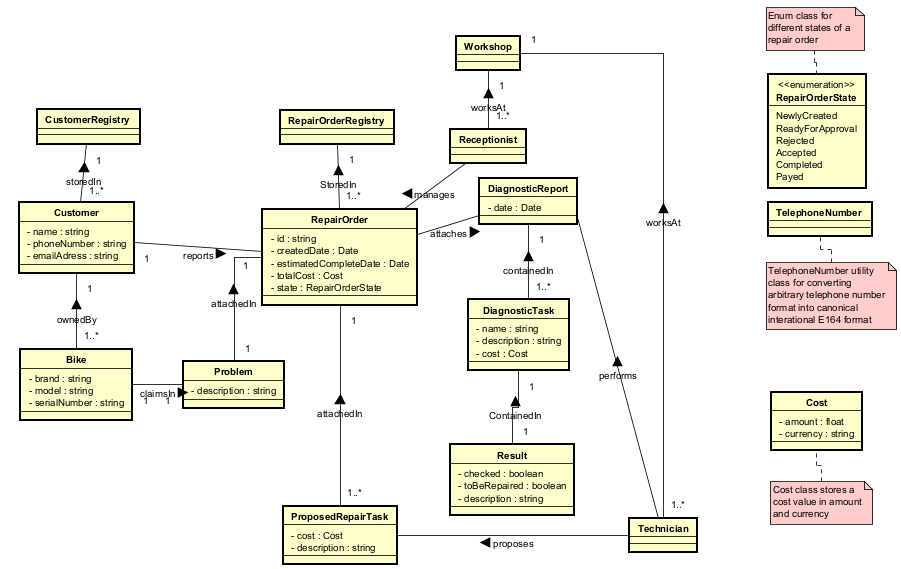
\includegraphics[width=\textwidth]{figures/domain-model.png}
    \caption{A domain model for the software system is shown. The connections between the entities shows their relationships.}
    \label{fig:domain-model}
  \end{center}
  
\end{figure}

\section{System sequence diagrams}
\label{appendix:system-sequence-diagram}
The repair electric bike scenario can also be summarized using a system sequence diagram that describe the basic and alternative flows. The basic flow can be visualized in Figure~\ref{fig:system-sequence-diagram}.

\begin{figure}[h!]
  \begin{center}
    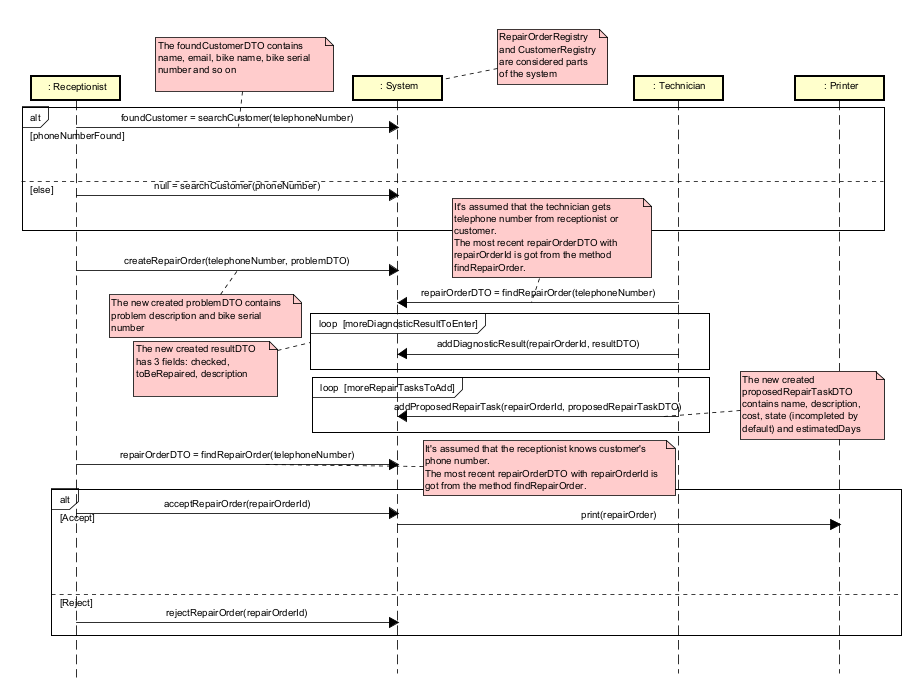
\includegraphics[width=\textwidth]{figures/system-sequence-diagram.png}
    \caption{The basic flow, as well as alternative flow is visualized in the system sequence diagram, where each real-world entity interact with the system using system operation. The intent is to enumerate the possible system operations.}
    \label{fig:system-sequence-diagram}
  \end{center}
  
\end{figure}

Alternative flows include invalid written telephone number and rejected repair order. Workflow for invalid telephone number can be visualized in Figure~\ref{fig:system-sequence-diagram}.

Both the domain model and system sequence diagram provide the analysis foundation for the software design. These diagrams describe the structure of the problem domain and the interactions between external actors and the system, and are therefore used for transforming the requirements specification into an object-oriented design according to the requirements. 

Since the requirements includes a layered architecture according to the Model-View-Controller (MVC) pattern as well as applying high coersion, low coupling and good encapsulation, all functionalities described in the requirements specification, including the basic workflow and alternative workflows are supported. Complete interaction diagrams that describe all system operations must therefore also be included, as well as a class diagram that represents all classes involved in the design.



\end{document}